
	In sections 2, 3 and 4, we have described the moduli space $\MM$ of flat $SU(2)$ connections on a compact Riemann surface $\Sigma$, and the corresponding spaces $P$ and $\cP$ of representations with weighted frames on $\Sigma$ and framed parabolic sheaves on $\tilde{\Sigma}$, a singular curve corresponding to $\Sigma$ via degeneration. Now in this section we will describe how this degeneration of $\Sigma$ to $\tilde{\Sigma}$ induces a degeneration of $\MM$ to $\cP$. This degeneration of moduli spaces is due to Biswas and Hurtubise \cite{biswas_degenerations_2021}. 
\section{Degeneration of the Curves}
	The relationship between the moduli spaces $\MM$ and $\cP$ is given by degenerating the Riemann surface $\Sigma$ to a nodal curve by smoothly shrinking the boundary curves of the trinion decomposition. First we describe a local model for this shrinking process.
	
	\begin{figure}[h]
		\centering
		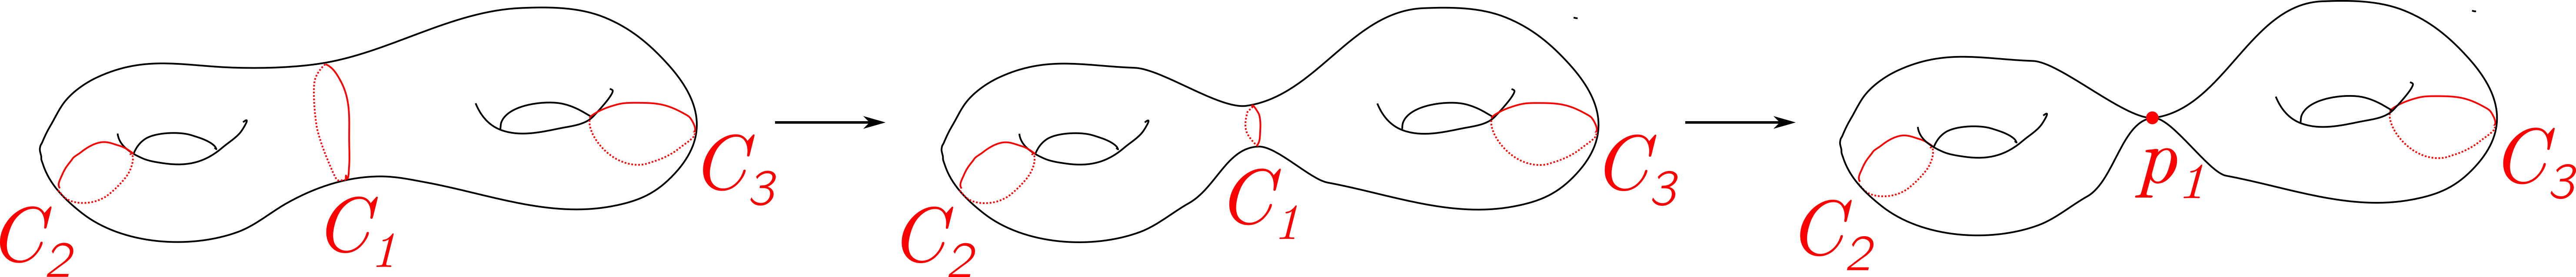
\includegraphics[width=0.6\linewidth]{degen1pt}
		\caption{Smoothly shrinking one boundary curve to a point.}
		\label{fig:degen}
	\end{figure}
	
	Let $\Sigma$ be a compact connected Riemann surface of genus $g$ as before. Let $\Sigma_0$ denote the nodal curve obtained by trinion decomposition from $\Sigma$, replacing each boundary circle of the trinions with a single point and then gluing at those points. Let $x_0 \in \Sigma_0$ be a nodal point corresponding to a boundary circle $C_0$. Let $\tilde{\Sigma}_0$ denote the desingularization of $\Sigma_0$. Let $x_1$ and $x_2$ denote the two points of $\tilde{\Sigma}_0$ which map to $x_0 \in \Sigma$. 
	
	Let $B$ be the polydisk in $\C^2$ given by the product of two disks of radius 2 centred at the origin. Then define a family $\QQ$ of quadrics for $t\in U$ by 
	\begin{equation}
		Q_t = \{(x,y)\in B\ ~|~ xy = t, t\in U\}.
	\end{equation}
	For $t=0$ we get the axes in $\C^2$ which is a local model for $\Sigma_0$ around $x_0$, and for $t \neq 0$ we get a cylinder which is a local model for $\Sigma$ on a tubular neighbourhood of the boundary circle $C_0$. For $t\neq 0$, the boundary of $Q_t$ is two circles, given by the equations
	\begin{align*}
		(x(t,\theta), y(t, \theta)) &= \left(
		2e^{i\theta}, \frac{t}{2}e^{-i\theta}
		\right)\\
		(x(t,\theta), y(t, \theta)) &= \left(
		\frac{t}{2}e^{i\theta}, 2e^{-i\theta}
		\right).
	\end{align*}
	There is a closed curve $c_t$ in $X_t$ given by
	\begin{equation}
		(x(t,\theta), y(t,\theta)) = \sqrt{t}(e^{i\theta}, e^{-i\theta}),
	\end{equation}
	which approaches $C_0$ at $t=1$ and $x_0$ at $t=0$. By gluing this local model to the boundaries of the disjoint union $(U\times S^1)\coprod (U\times S^1)$ one obtains a family over $U$, with fibre $\Sigma_0$ at $t=0$, and $\Sigma \cong \Sigma_t$ (topologically) at $t\neq 0$.

\section{Local Model for the Connections}
	\label{s:local-model-conns}
	On our local model for the degeneration of the curve $\Sigma$, one also has a local model for the degeneration of a unitary connection $\nabla$ on a vector bundle $E$ over $\Sigma$. Theorem \ref{t:atd-thm} guarantees that there exists some $\alpha \in \mathfrak{t}$ such that locally,
	\begin{equation}
	\nabla = d + i\frac{\alpha}{2}(d\theta_x - d\theta_y) = \partial + \frac{\alpha}{4}\left(\frac{dx}{x}-\frac{dy}{y}\right) + \dbar+ \frac{\alpha}{4}\left(\frac{d\bar{x}}{\bar{x}}-\frac{d\bar{y}}{\bar{y}}\right),
	\end{equation} 
	where $\theta_x$ and $\theta_y$ are the arguments of the complex co-ordinates $x$ and $y$. The holonomy $C := \Hol_{c_1}(\nabla)$ will be given in this gauge by $C = e^{-2\pi i \alpha}$. On our family $Q_t$, this connection is well defined for all $t\neq 0$, and it is isomonodromic, meaning that for all $t\neq 0$, 
	\begin{equation}
	\Hol_{c_t}(\nabla) = \Hol_{c_1}(\nabla)=C.
	\end{equation}
	It remains to describe the connection in the limit $t=0$. Change co-ordinates on $Q_t$ from $(x,y)$ to $(x,t)$, and the connection becomes
	\begin{equation}
		\nabla = d + i\frac{\alpha}{2}(2d\theta_x - d\theta_t).
	\end{equation}
	Similarly in co-ordinates $(y,t)$ we have
	\begin{equation}
		\nabla = d + i\frac{\alpha}{2}(-2d\theta_y + d\theta_t).
	\end{equation}
	Since $Q_t$ is defined by the equation $xy=t$, $d\theta_t$ is a normal component and one may project it out to obtain a partial connection $\nabla^p$ on $Q_t$. On the patch $x\neq 0$, using $x$ co-ordinate:
	\begin{equation}
		\label{e:dtx}
		\nabla^p = d + i\alpha d\theta_x.
	\end{equation}
	This extends well to the limit $y\to 0$, despite the original connection $\nabla$ having a singularity. On the patch $y\neq 0$ with $y$ co-ordinate:
	\begin{equation}
		\label{e:dty}
		\nabla^p = d - i\alpha d\theta_y,
	\end{equation}
	which also passes well to the limit $x\to 0$. Therefore we obtain a partial connection $\nabla^p$ defined everywhere on $Q_0$ except the nodal point $x_0$. 
	
	This local model can also be described in terms of the holonomy of the connection. Suppose first that $\Sigma - c_1$ is not disconnected \footnote{A similar analysis can be performed for disconnecting curves, see \cite[Page 10]{biswas_degenerations_2021}.}, and denote by $\tilde{\Sigma}_0$ the desingularized degenerated curve. In this case, $\tilde{\Sigma}_0$ has genus $g-1$. Let $p_1, p_2$ denote the punctures in $\tilde{\Sigma}$ corresponding to $c_0 = x_0$. Then $\tilde{\Sigma}$ is a twice punctured curve for which we have the extended moduli space $\MM^G$ from section \ref{s:mastermoduli}:
	\begin{equation}
		\MM^G = \left\{\left((A_i,B_i)_{i=1}^{g-1}, (C_1,C_2,D_1,D_2)\right), ~|~ \prod_{i=1}^{g-1}[A_i,B_i]D_1C_1D_1^{-1}D_2C_2D_2^{-1} = 1\right\} / SU(n)
	\end{equation}
	On the original space $\Sigma$, the connections correspond to representations of $\pi_1(\Sigma)$; picking a point $p\in\Sigma$, let $d_1$ and $d_2$ be curves from $p$ to $c_1$ such that $d_1d^{-1}_2$ is a non-contractible loop based at $p$. Then let $(A_i,B_i)_{i=1}^{g-1}$ denote the standard generators for the rest of $\pi_1(\Sigma)$. In this notation, a connection on $\Sigma$ is represented by holonomies $\left((A_i,B_i)_{i=1}^{g-1}, C,D_1,D_2\right)$ around these curves.
	
	Applying the degeneration, the resulting connection on $\tilde{\Sigma}_0$ has holonomy $C$ around the puncture $p_1$ and $R(C)^{-1}$ around the puncture $p_2$, where $R$ reverses the order of the entries of $\alpha$. Gluing $p_1$ and $p_2$, the fundamental group of the result $\Sigma_0$ has the relation
	\begin{equation}
	 D_1^{-1}CD_1D_2^{-1}C^{-1}D_2 = 1, \implies D_2D_1^{-1}CD_1D_2^{-1} = C.
	\end{equation}
	Therefore, $D_1D_2^{-1} \in \Stab(C)$, or $D_1\mu = D_2$ for some $\mu\in \Stab(C)$. Our local degeneration thus sends the connection $\nabla = (A_i,B_i,C,D_1,D_2)$ on $\Sigma$ to the orbit
	\begin{equation}
		\label{e:degen-action}
		(A_i,B_i,C,D_1,D_2) \to \left(
		(A_i,B_i), (\mu C \mu^{-1}, D_1, D_1 \mu)\right), ~\mu \in \Stab(C)
		= \text{Orb}_{\Stab (C)} (\nabla),
	\end{equation}
	in $\MM^G$. If $C$ is in $\exp \Delta^0$, then $\Stab(C) = \{e\}$ and the degeneration is bijective. Otherwise, when $C = \pm 1$, then $\Stab(C) = SU(2)$. Notice that the action of equation \ref{e:degen-action} matches the action of the $k$-th copy of $G$ on $\MM^G$ of equation \ref{e:impl-action}. Therefore, these orbits are points in the strata of the imploded cross-section of $\MM^G$. When we perform this local degeneration for each curve in the trinion decomposition, which corresponds to imploding $\MM^G$ for each puncture, we will obtain an element in the imploded cross-section $P$. 
 	
\section{Degeneration of the Moduli Space}
	Using this local model, one can describe the degeneration of the entire moduli space $\MM$ as $\Sigma$ is degenerated to $\Sigma_0$. First we will describe the degeneration in terms of representations of $\pi_1(\Sigma)$, and we will see that $\MM$ degenerates to obtain $P$.
	
	Consider the connected genus $g$ surface $\Sigma$ and its desingularized degeneration $\Sigma_0$. Let $\{c_i\}_{i=1}^{3g-3}$ be boundary curves in a trinion decomposition for $\Sigma$, which degenerate to points $\{p_i\}_{i=1}^{6g-6}$ in the desingularized curve; $p_{2k-1}$ and $p_{2k}$ each come from the degeneration of the curve $c_k$. 
	
	On $\Sigma_t$ for $t\neq 0$, we simply have the moduli space $\MM_t$ of flat $SU(2)$ connections which corresponds to the moduli space of stable holomorphic vector bundles with $SL(2,\C)$ structure over $\Sigma_t$. Therefore it remains to understand the moduli space over $\Sigma_0$ and the desingularisation $\tilde{\Sigma}_0$. 
	
	Let $p$ be a nodal point in $\Sigma_0$ and $x_1,x_2$ the two points in $\tilde{\Sigma}_0$ which correspond to $p$. Any connection on $\Sigma_0$ has holonomy $A_i\in SU(2)$ around each nodal point which lives in the fundamental alcove of $SU(2)$. We can write the alcove as
	\begin{equation}
		\cA = \{\exp\left(
		-2\pi i ~\text{diag}(\gamma, -\gamma)
		\right)~|~ \gamma \in[1/2,1]\},
	\end{equation}
	and the logarithms of the holonomies are the values of $\gamma$. Under the Mehta-Seshadri correspondence these logarithms will define the weights for a parabolic structure of the $SL(2,\C)$ bundle corresponding to the connection. The flags assigned to the points $x_1$ and $x_2$ will be determined by the eigenspaces of $A_i$.
	
	Let $\Delta = [1/2,1]$, which divides into three faces $\{1/2\}, \{1\}$ and $(1/2,1)$. When $\gamma \in (1/2,1)$, the corresponding holonomy matrix has two distinct eigenvalues $\gamma$ and $-\gamma$.  If $\gamma=1/2$ then $A_i = -\mathds{1}$, and if $\gamma = 1$ then $A_i = \mathds{1}$.
	
	Fix $\gamma \in [1/2,1]$ and consider the space of connections with holonomy whose logarithm is $\gamma$ about $p_i$. Quotienting out the gauge choice of $SL(2,\C)$ framing around $p_i$, the Mehta-Seshadri theorem \cite{mehta_moduli_1980} tells us that this space of connections corresponds to the holomorphic moduli space of parabolic $SL(n,\C)$ vector bundles $E$ with parabolic structure at $p_i$ of weight $\gamma$. The parabolic structure is the flag given by the largest eigenspace of the holonomy, i.e. that with eigenvalue $\gamma$. When $\gamma = 1/2$ or $1$, then we acquire instead a framed parabolic sheaf with torsion at $p_1$ and the $SL(2,\C)$ structure vanishes, as discussed in section \ref{s:mastermoduli}.
		
	To obtain the entire moduli space of connections on $\Sigma_0$ and $\tilde{\Sigma}_0$, we need to allow the weights to vary and fit the space for each weight together. This was the construction of $\cP$ from section \ref{s:mastermoduli}, the space of framed parabolic sheaves constructed by Hurtubise and Jeffrey. In summary, we have \cite[Theorems 3.17, 4.1]{biswas_degenerations_2021}
	\begin{theorem}[Biswas and Hurtubise]
		\label{t:bishurt}
		There is a fibre bundle $\pi: \XX \to \C$, for which
		\begin{itemize}
			\item $\pi:\XX\to \C$ is a flat family of irreducible reduced schemes.
			\item For any $t\in \C^\ast$, the fibre $X_t = \pi^{-1}(t)$ is isomorphic to $\MM$.
			\item The special fibre $\pi^{-1}(0)$ is $\cP$, which is a toric variety.
		\end{itemize}
		We refer to this bundle as the \emph{degeneration of $\MM$ to $\cP$}, or simply \emph{the degeneration}.
	\end{theorem}
	We can rephrase this degeneration as a surjective map $\phi:\MM\to P$, given by taking an element $A\in X_1 \cong \MM$ to its corresponding degenerated element $A_0 \in X_0 \cong P$, given locally by the model in section \ref{s:local-model-conns}. In terms of the extended moduli spaces of section $\ref{s:mastermoduli}$, $\phi$ is the composition of the inclusion and quotient maps:
	\begin{equation}
		\MM = \MM^T \hookrightarrow \MM^G \twoheadrightarrow P,
	\end{equation}
	described by Hurtubise and Jeffrey \cite[prop 2.37]{hurtubise_representations_2000}. 
	\begin{lemma}
		Given an element $A\in \MM$, let $D(A)$ denote the element in $P$ obtained by performing the local degeneration of section \ref{s:local-model-conns} at each curve in a trinion decomposition for $\Sigma$. Then $D(A) = \phi(A)$, where $\phi(A)$ is the composition of maps 
		\begin{equation}
			\MM = \MM^T \hookrightarrow \MM^G \twoheadrightarrow P,
		\end{equation}
		where the surjection is the quotient map of the imploded cross-section.
	\end{lemma}
	\begin{proof}
		Fix one closed curve $\gamma_k$ in the trinion decomposition. Then an element $A\in \MM$ defines a holonomy $C_k\in T\subset SU(2)$ around $\gamma_k$, and we also have the local model for the degeneration $D(A)$ on a tubular neighbourhood around $\gamma_k$. First let us compute $\phi(A)$. Suppose $A = (A_i,B_i,C_j,D_j)$. Then to compute the quotient for the imploded cross-section, we have three faces $\{\sigma_0, \sigma_+, \sigma_-\}$ of $\Delta = [0,1]$ to consider. If $C_j^{-1} \in \exp \sigma_0$ then it is quotiented by the stabiliser $[G_\sigma,G_\sigma] = \{e\}$ as discussed in section \ref{s:mastermoduli}. If $C_j^{-1} = \pm 1$, then it is quotiented by the stabiliser $[G_\sigma, G_\sigma] = G$, under the action
		\begin{equation}
			D_k \to D_k g^{-1},~ C_l \to g C_l g^{-1}.
		\end{equation}
		In summary:
		\begin{equation}
			\phi(\nabla) = \begin{cases}
				(A_i,B_i,C_j,D_j), & C_k \in \sigma_0\\
				\text{Orb}_{SU(2)}(\nabla) , & C_k \in \sigma_\pm
			\end{cases}
		\end{equation}
		On the other hand, the degeneration $D(A)$ takes $(A_i,B_i,C_j,D_j)$ to the set
		\begin{equation}
			D(A) = \left\{
			\left(
			(A_i,B_i,C_j,D_j)_{j\neq k} (C_k, D_k, D_k\mu) ~|~ \mu \in \Stab(C_k)
			\right)
			\right\}
		\end{equation}
		For $C_k$ in $\sigma_0$, the stabilizer is $\{e\}$ and we have
		\begin{equation}
			D(A_i,B_i,C_j,D_k) = (A_i,B_i,C_j,D_k) = \phi(A).
		\end{equation}
		If $C_k$ is in $\sigma_\pm$, then the stabilizer is $SU(2)$ and we have
		\begin{equation}
			D(A_i,B_i,C_j,D_k) = \text{Orb}_{SU(2)}(\nabla),
		\end{equation}
		under the action of $SU(2)$ of equation \ref{e:impl-action} which is the same as that defined for the imploded cross-section. Hence on each stratum, $\phi(\nabla) = D(\nabla)$. 
		
		For each curve in the trinion decomposition, we can repeat this process, until it remains to perform the final quotient by the first copy of $G$. After these implosions, we arrive at the set
		\begin{equation}
			\left\{
			(C_1,W_2,...,W_n) ~|~ C_1 \in G, W_j \in D(G)_{impl}, C_1\prod_{j=2}^{n}\Phi_G(W_j) = 1	
			\right\}. 
		\end{equation}
		Where $W_j = (D_j,C_jD_j) \in D(G)_{impl}$, $j\neq 1$ and $W_1 = (\mathds{1},C_1)$. The final copy of $G$ acts by (Equation 4.15)
		\begin{equation}
			g\cdot(W_1,...,W_{n}) = (C_1,gD_2,C_2,...,gD_n, C_n). 
		\end{equation}
		As for the degeneration $D$, the final copy of $G$ acts by global conjugation on the representations $\Hom(\pi_1(G),G)$. However, as we already fixed the connection $A$ to be in A.T.D. gauge, we know $C_j \in T$ and hence the conjugation action fixes $C_j$, and is given by
		\begin{equation}
			g \cdot (C_1,(C_j,D_j, D_j\mu)_{j=2}^n) = (C_1, (C_j, gD_j, gD_j\mu)_{j=2}^n),
		\end{equation}
		which agrees with the action for the implosion. 
	\end{proof}
	
	\section{Toric Degenerations}
	Here we want to describe a result of Harada and Kaveh (cite), which constructs an integrable system from a \textit{toric degeneration} satisfying some additional hypotheses. 
	\begin{definition}
		\label{d:toricdegen}
		Let $X$ be an $n$-dimensional quasi-projective irreducible reduced scheme. We call $\pi: \XX\to\C$ a \emph{toric degeneration} of $X$ if:
		\begin{enumerate}
			\item $\pi:\XX\to\C$ is a flat family of irreducible reduced schemes.
			\item The family $\XX$ is trivial over $\C^\ast$, namely there exists a fibre-preserving isomorphism $\rho:X\times\C^\ast \to \XX - X_0$, such that for each $t\in \C^\ast$ $\rho_t:X\times\{t\} \to X_t$ is an isomorphism.
			\item The fibre $X_0$ is a toric variety with respect to an action of $(\C^\ast)^n := \mathbb{T}$.
		\end{enumerate}
	\end{definition}
	Theorem \ref{t:bishurt} tells us that in this case, the moduli space $\MM$ of flat $SU(2)$ connections serve as our quasi-projective scheme, and we have a toric degeneration to the moduli space of parabolic sheaves $\cP$. Now let us describe the additional hypothesis that are required for Harada and Kaveh's result.
	
	Suppose $\pi:\XX\to\C$ is a toric degeneration of $X$, and $X$ has a Kahler form $\omega$. Let $\Omega$ denote a constant multiple of a Fubini-Study Kahler form on $\mathbb{P}^N$, and equip $\mathbb{P}^N\times\C$ with the Kahler structure $\Omega \times \omega_{std}$. Assume that:
	\begin{enumerate}
		\item The family $\XX$ is smooth away from the zero fibre $X_0$.
		\item The family $\XX$ is embedded in $\mathbb{P}^N\times \C$ as an algebraic subvariety, for some projective space $\mathbb{P}^N$ such that:
		\begin{itemize}
			\item the map $\pi:\XX\to\C$ is the restriction of $\XX$ to the projection of $\mathbb{P}^N\times \C$ to $\C$;
			\item the action of $\mathbb{T}$ on $X_0$ extends to a linear action on $\mathbb{P}^N$.
		\end{itemize}
		Let $\omega_t$ denote the restriction of $\Omega\times \omega_{std}$ to the fibre $X_t$ embedded in $\mathbb{P}^N \times {t}$. Then
		\item The map $\rho_1 : X\to X_1$ is an isomorphism of Kahler manifolds; $\rho_1^\ast(\omega_1) = \omega$;
		\item Let $T = (S^1)^n$ denote the compact subtorus of $\mathbb{T}$. The Kahler form $\Omega$ on $\mathbb{P}^N$ is $T$-invariant and in particular the restriction $\omega_0$ to the toric variety $X_0$ is a $T$-invariant Kahler form.
	\end{enumerate}
	Given a toric variety satisfying these conditions, Harada and Kaveh provide the following theorem:
	\begin{theorem}[Harada and Kaveh]
		\label{t:haradakaveh}
		Let $\pi:\XX\to \C$ be a toric degeneration of $X$, and let $\omega$ be a Kahler structure on $X$. If $\pi:\XX\to\C$ satisfies conditions 1-4 above, then:
		\begin{enumerate}
			\item There exists a surjective continuous map $\phi:X\to X_0$ which is a symplectomorphism restricted to a dense open subset $U\subset X$.
			\item There exists a completely integrable system $\mu = (F_1,...,F_n)$ on $(X,\omega)$ whose moment polytope $\Delta$ coincides with the moment polytope of $(X_0, \omega_0)$.
			\item Let $U\subset X$ be the open dense subset of $X$ from item 1. Then the integrable system of item 2 generates a Hamiltonian torus action on $U$, and the inverse image $\mu^{-1}(\Delta^\circ)$ of the interior of $\Delta$ under the moment map lies in the open subset $U$.
		\end{enumerate}
	\end{theorem}

	\section{Degeneration of the Moduli Space over one Trinion}
	The local model for our degeneration gives us a description of the degeneration of the moduli space $\MM(D) \to P(D)$ for a single trinion $D = S^2 - {p_1,p_3,p_3}$. Let $B$ be the polydisk in $\C^2$ given by the product of two disks of radius 2 centred at the origin, and $U$ the unit disk in $\C$. As before, we can define a family for $t\in U$ by
	\begin{equation}
		Q_t = \{(x,y)\in B ~|~ xy = t, x\geq y, t\in U\}.
	\end{equation}
	By requiring $x\geq y$, we are taking only half of the local model for the curve that we had before. For $t=0$, the space $Q_0$ becomes a punctured disk, which is a local model for $D$ in a neighbourhood of one of the punctures $p_i$. Now, restricting all the discussion of our local connections in section $\ref{s:local-model-conns}$ to $Q_t$, we get that a connection
	\begin{equation}
		\nabla = d + i\frac{\alpha}{2}(d\theta_x - d\theta_y)
	\end{equation}
	on $Q_1$ degenerates to a connection
	\begin{equation}
		\nabla' = d + i\alpha d\theta_x
	\end{equation}
	on $Q_0$. Given two trinions $D_1$ and $D_2$ which we wish to glue together at the punctures $p_1$ and $q_1$, let $Q_{0,1}$ and $Q_{0,2}$ be local models around $p_1$ in $D_1$ and $q_1$ in $D_2$ respectively. If we let $Q_{0,1}$'s co-ordinate be $x$ and $Q_{0,2}$'s co-ordinate be $y$, we see that $Q_{0,1}\cup Q_{0,2}$ agrees with our local model for the desingularized degenerated curve $\tilde{\Sigma}$ around the glued points. That is:
	\begin{equation}
		Q_{0,1}\cup Q_{0,2} = \{(x,0)\in B~|~ x\neq 0 \}\cup {(0,y)\in B~|~ y\neq 0} = \{(x,y)\in B~|~ xy=0\} 
	\end{equation}
	Given connections
	\begin{align*}
		\nabla_1 &= d + i\alpha d\theta_{x_1}, & \nabla_2 &= d + i\beta d\theta_{x_2}
	\end{align*} 
	on $Q_{0,1}$ and $Q_{0,2}$, equations (\ref{e:dtx}) and (\ref{e:dty}) tell us that $\nabla_1$ and $\nabla_2$ are in the image of the degeneration if $\alpha = -\beta$. 